\section{Methodology}
\label{sec:methodology}

\begin{figure*}[t]
    \centering
    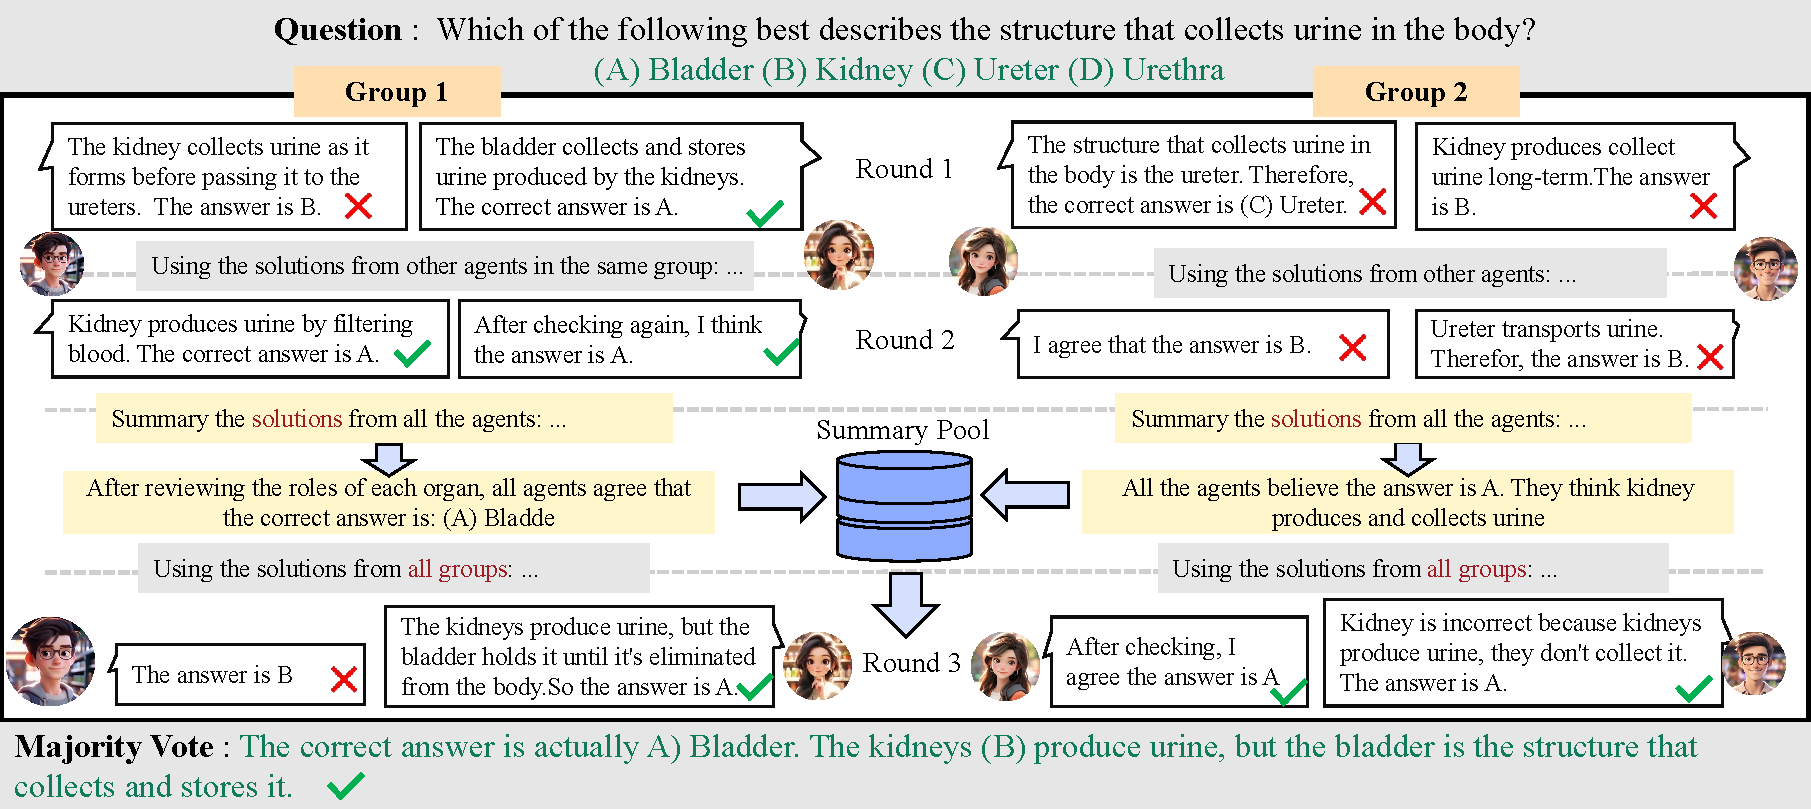
\includegraphics[width=1\linewidth]{figs/GroupDebate.pdf}
    \caption{\textbf{An Example of GroupDebate.} 4 agents are divided into 2 groups and the GroupDebate process comprises two stages, with each stage involving two rounds of intra-group debate.}
    \label{fig4}
    \vspace{-0.5cm}
\end{figure*}

In this section, we first introduce the overall framework of our GroupDebate. Subsequently, we provide mathematical analysis of the token cost for both MAD and our GroupDebate. Formally, assume there are $M$ LLM-based agents, denoted as $A=\{A_i | i=1,2,\cdots,M\}$, participating in a multi-round debate, with the total number of debate rounds denoted as $T$. In each round $t$ $(t=1,2,\ldots,T)$, the output of each agent $A_i$ is represented as $Output_i^{t}$. These outputs are dynamically refined through structured inter-agent interactions, where agents critique, verify, and build upon reasoning from others. The tokens of the initial question prompt are denoted as $Q$, serves as the foundational query propagated through the debate process. These notations will be used throughout this paper.

\subsection{GroupDebate} 
\label{multi-agent-group-debate}

The GroupDebate framework orchestrates collaborative reasoning among 
M LLM-based agents, denoted as $A=\{A_i | i=1,2,\cdots,M\}$, which can be randomly divided into $N$ groups $G=\{G_j|j=1,2,\cdots,N\}$, with average K agents in each group. 
The GroupDebate splits the total debate rounds into $S$ stages, with each stage encompassing $R$ rounds. Thus, the total number of rounds $T$ can be calculated as $T=S\times R$. This hierarchical design enables efficient exploration of solution spaces through alternating phases of localized refinement (intra-group) and global synthesis (inter-group).
For the $s$-th stage's $r$-th round, GroupDebate selects one of the following processes:
\begin{enumerate}
\item[(1)] \textbf{Initial Thinking.} If $s=1$ and $r=1$ (i.e., the first stage's first round), we input the initial question prompt $Q$ to each agent.
\item[(2)] \textbf{Intra-group Debate.} If $r>1$, we utilize the outputs from other agents within the same group as the input for each agent.
\item[(3)] \textbf{Inter-group Debate.} If $s>1$ and $r=1$, we merge the outputs from the last round of each group into a summary and input the summaries from other groups to each agent.
\end{enumerate}


Meanwhile, inspired by \cite{sun2023corex}, we summarize the responses from other groups and restrict each agent to receive the latest summary from the previous stage in the inter-group debate.
After the $S$-th stage's $R$-th round, all agents vote, and the ultimate result is determined by the majority selection. The detailed GroupDebate process can be found in Appendix \ref{appendix:gd-al}. The Figure \ref{fig4} illustrates an example of GroupDebate consisting of two stages and two groups. In the first stage, two agents in each group receive the initial question and exchange ideas within the group. In the second stage, agents share the summaries of their respective groups between groups and then discuss within their own groups again.

% \begin{figure*}[t]
%     \centering
%     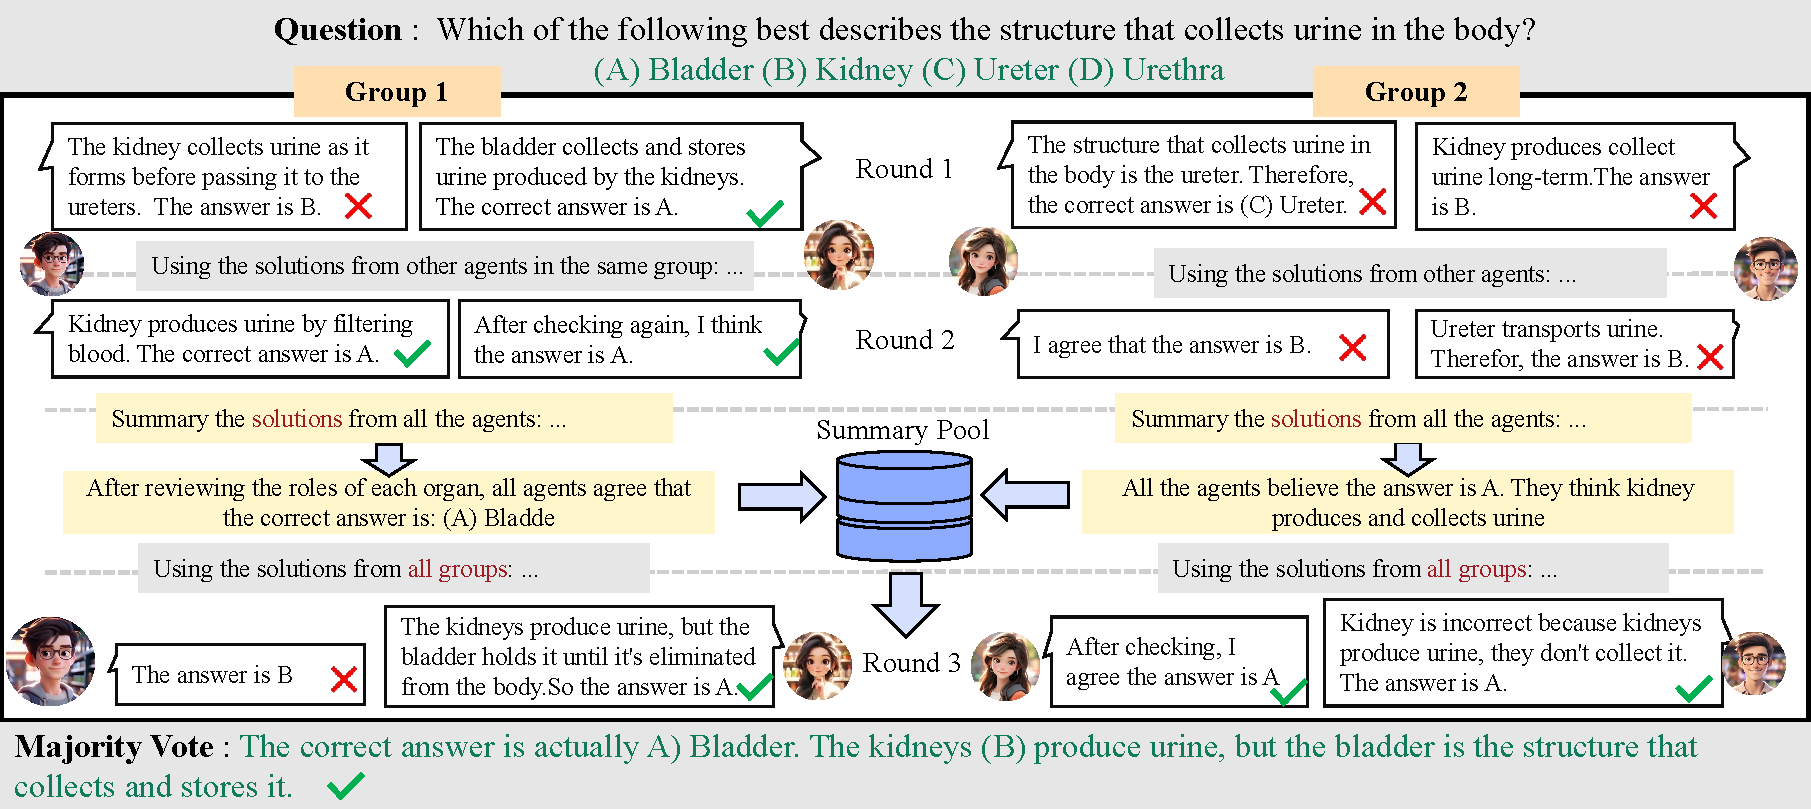
\includegraphics[width=1\linewidth]{figs/GroupDebate.pdf}
%     \caption{\textbf{An Example of GroupDebate.} 4 agents are divided into 2 groups and the GroupDebate process comprises two stages, with each stage involving two rounds of intra-group debate.}
%     \label{fig4}
%     \vspace{-0.5cm}
% \end{figure*}

\subsection{Token Cost Analysis} \label{token-consumption-analysis}

\paragraph{Token Cost in Multi-agent Debate.} 

We implement the summary mechanism in MAD following \cite{du2023improving}, where the output of other agents is summarized and used as input for each agent in the next round. The summary for agent $A_i$ in round $t$ is denoted as $Summary_i^t$. 
Then token cost $Token^t$ in each round $t$ can be computed as follows:

\begin{equation}
\begin{split}
% Token^t=
\left\{
\begin{aligned}
& \sum_{i=1}^M (Q+Output_i^t),   &&{t=1} \\
& Token^{t-1}+\sum_{i=1}^{M}(S_{i}^{t-1}+  Output_{i}^{t}),   &&{t>1}
\end{aligned}
\right.
\end{split}
\end{equation}
Finally, the total token cost in MAD is 
\begin{align}
Token^{GD} = \mathcal{O}\left( MTQ+(M^2T+MT^2)C \right)
\end{align}
where $C$ represents the upper bound on the token number for each agent's response and the generated summary. More mathematical details are illustrated in Appendix \ref{appendix:token-cost-mad}.
%$Token^{MAD} = \mathcal{O}\left( MTQ+(M^2T+MT^2)C \right)$, where $C$ represents the upper bound on the token number for each agent's response and the generated summary. More mathematical details are illustrated in Appendix \ref{appendix:token-cost-mad}.

\paragraph{Token Cost in GroupDebate.} In GroupDebate, we summarize the outputs from other groups at the end of each stage. Here, we define the summary of group $G_j$ at the end of stage $s$ as $Summary_j^s$. 

Then token cost $Token^t_s$ in round $t$ at stage $s$ is:

Then the token cost in the intra-group debate is:
\begin{equation}
    \sum_{j=1}^N \sum_{i\in G_j} (Q+Output_i^{t}+ \sum_{i'\in G_j} Output_{i'}^{t-1}),
\end{equation}
where $(s-1)R+1<t<=\min(sR,T)$. The token cost in the inter-group debate is:
% \begin{equation}
\begin{multline}
    \sum_{i=1}^{M} (Q + Output_i^{t-1} + \sum_{j=1}^{N} Summary_j^{s-1} + Output_i^{t}),
\end{multline}
% \end{equation}
where $t=(s-1)R+1$.
Finally, the total token cost of GroupDebate is $Token^{GD} = \mathcal{O}\left(MTQ+(\frac{M^2T}{N}+MSN)C\right)$, where $C$ represents the upper bound on the token number for each agent's response and the generated summary. More calculation details are shown in Appendix \ref{appendix:token-cost-gd}.

\begin{figure*}[t]
    \centering
    \includegraphics[width=1\linewidth]{figs/5.pdf}
    \caption{\textbf{Comparison of Token Cost and Accuracy Between GD and MAD under Different Agents and Rounds.} The notation (5,4) signifies 5 agents with 4 rounds. The results are average.}
    \label{fig5}
    % \vspace{-0.5cm}
\end{figure*}

\paragraph{Discussion.} From the perspective of overall token cost complexity, GD and MAD exhibit the same level of complexity regarding the input token cost of the question prompt $Q$, indicating that the question prompt has an equal impact on both methods. In our GroupDebate, given fixed values for $T$ and $M$, the number of groups $N$ and the total number of stages $S$ can be dynamically adjusted. When we set $N \rightarrow \mathcal{O}\left(\sqrt{\frac{MT}{S}}\right)$, theoretically, we can obtain $Token^{GD} \rightarrow \mathcal{O}\left(MTQ+\sqrt{M^3TS}C\right)$. This complexity is significantly lower than that of MAD. If we consider setting $S$ to a small positive integer, treating it as a constant, then $Token^{GD}$ can further approach $\mathcal{O}\left(MTQ+\sqrt{M^3T}C\right)$. Moreover, $N$ and $S$ also influence the diversity in multi-agent debate, affecting the accuracy of the debate results, which will be further studied in Section \ref{hyperparameter-study}.
